\documentclass[11pt, journal]{IEEEtran}

\usepackage[pdftex]{graphicx}
\usepackage[margin=1in]{geometry}
\usepackage{fancyhdr}

\begin{document}
\title{Fancy title here}

\author{Harsh~Damania, Christophe~Faucon, Nicolas~Salhuana, Tsung-Yen~Yu}

\IEEEcompsoctitleabstractindextext{%
\begin{abstract}
The abstract goes here.
\end{abstract}

\begin{IEEEkeywords}
social networking, location services, clustering
\end{IEEEkeywords}}

\maketitle
\IEEEdisplaynotcompsoctitleabstractindextext

\section{Introduction}
	\IEEEPARstart{I}{n} today's day and age where technology keeps changing and new ideas are born on a daily basis, there are still a lot of holes left to plug in various areas of computing. There has been a tremendous success of mobile apps in the areas of social networking and location based services, and there have been quite a few that combine these 2 disciplines. Our project provides a little a twist to these 2 disciplines to make it different from other apps, and make it better for people on the go.

	\subsection{Project Description}
		Our project is location based social network. There can a lot be done with a users location, and thus we chose to use this location data to group a user within a zone with other app users. The size of the zone is determined by the number of other app users around. While in a zone, the user can then send messages to others within the same zone and discuss and what's happening near by. This app would help users understand if there is something special on nearby, and also help understand the events in the zone.
	
	\subsection{The Need}

		The main use of the app would be for the social networking and getting to know what is going on around you at a given time. There have been a number of other mobile apps that have gained traction lately that relate to social networking and location based services, but none quite have a good blend of the 2 that can be used on the go.

		The use of a location service where a user is automatically allocated to a zone they are in based on ``hotspots''. This way a user who is new to the area can instantly tell what is going on at the moment based on where other app users are and see if there is anything special going on.

		Another noteworthy use of the app is for getting a live feed of the current event in a ``hotspot''. For example, for a college football game, there could be a large number of users in around the stadium that form a zone and everyone within that zone can talk and discuss about the game on that thread. Users are stored within a zone 24 hours after they have left it if they wanted to discuss the thread for a little while after the event too.

\section{Related Work}
There is a wide variety of mobile social networks that are available for different platforms. These social networks range from being ubiquitous (Facebook, Instagram, Snapchat, Twitter, etc.) to incredibly niche (targeting cat lovers, etc.). After researching the rise of various large social networks, we have seen that most of them started off in the niche social network category. Facebook is a prime example of this. It is currently the largest social network in the world but it started off as only a minute target audience. In the beginning, Facebook only allowed users with a Harvard.edu email address to sign up for their social network. They then expanded and have become an incredibly successful publicy traded company.
The current trend in mobile social networks has been leaning towards finding that initial niche. This has varied from the previously mentioned animal lover groups to the athletic groups. A new trend that has started to take place over the past year is forming groups by localization. The thought process behind this is that you are bound to have common interests by the sheer nature of being in the same vacinity as the other people you are connected with. The most popular localization mobile social network out right now is Yik Yak. In Lehman's terms, it is an app similar to Twiiter that replicates Twitter's short message feed. The way it differs is that user's cannot follow other users. The posts are either anonymous or with a creative username that doesn't have to be persistent to that user. Users only see messages (called "Yaks") that are posted within a two-mile radius. This app was released within the past year and is currently active at over 1,000 college campuses around the US. Yik Yak was also able to secure a $300 million valuation two weeks ago. 
Location-based social networks are not a completely new concept. The paper that we presented on was proposing a location-based mobile social network, E-Small Talker. This app was different than Yik Yak for a variety of reasons. E-Small Talker was attempting to enhance the connection between one user to another user whereas Yik Yak is for a group of users in a predefined area. E-Small Talker would connect with other users using Bluetooth and using Bloom Filters would figure out the common interests between the users. The app would then alert both users and conversation would flow smoothly. This app had a low chance of success. Since Bluetooth's range is so limited, the app would have to be widely adopted and reach critical mass to give the users the intended effect.
For our app, we looked at various successes that the larger social networks have had while also looking at how the niche networks began to gain traction. We expanded on the idea of a group of users able to interact within a given distance of each other. We changed the hard coding of 2.5 miles that Yik Yak uses and implemented our own algorithm to build around popular zones. 

\section{Goals}
	For our project, we had 3 main goals that we wanted to accomplish
	\begin{itemize}
		\item Ability for the user to be assigned a zone automatically based on location: We wanted to make sure that the user would be allocated into their zone based on where the other app users were. This further determined zones for future users to connect to. This was the heart of the project.
		\item Users should be able send messages to others in their zones: The entire point of being allocated in a zone is for the users to see what others around them are discussing. Since this is a part social network, it is integral for the user to communicate with others.
		\item Setup a centralized server with Zone messages: Our project will rely on a centralized service that a user can GET and POST to. Joining a zone, downloads the messages on to the users device.
	\end{itemize}

\section{System Model and Problem Statement}

\subsection{System Model}
\begin{figure}
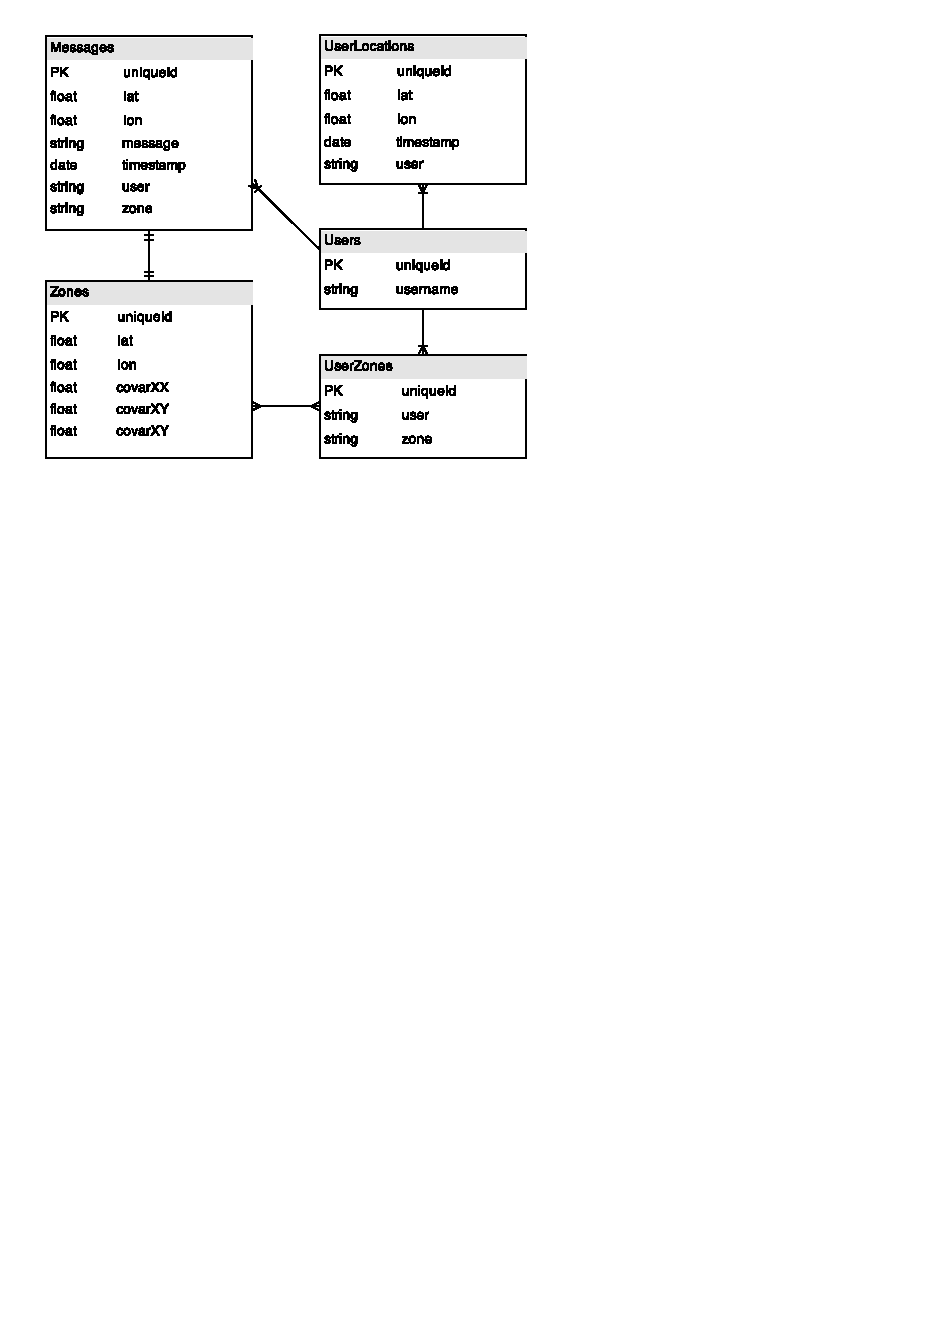
\includegraphics{figs/systemModel}
\caption{GeoChat Database structure.  The user pings the server regularly with their location which is used to determine which zones they should be a part of, and which messages they can see.  Zones behave much like geo-spatial conversation threads, where all messages are public within them.  Zone covariance defines the size and shape of the zones.}
\label{systemModel}
\end{figure}

Our system was implemented with a relatively simple database model shown in figure~\ref{systemModel}.  Firebase allows developers to watch one key on a table for instantaneous updates, and for this reason it is critical to ensure that we can indicate whether a message will be relevant to a user with a single key.  To this end we reorganized our code so that instead of watching a pair of lat/long co-ordinates we instead watch a particular zone.  The zones are calculated by expectation maximization of a gaussian mixture model, discussed in the implementation section.

\subsection{Problem Statement}
Terms, definitions, components


\section{Approach}

	\subsection{Idea}

	\subsection{Planned Architecture}

	\subsection{Implemented Architecture}

\section{Implementation}
\begin{figure}
\fbox{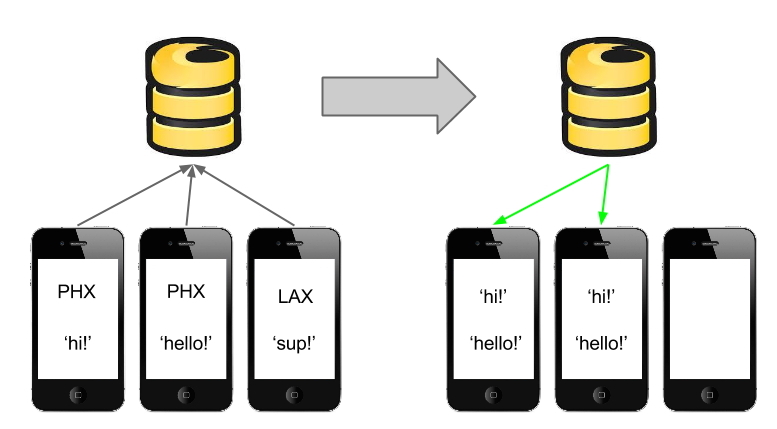
\includegraphics[width=.48\textwidth]{figs/chatExample}}
\caption{Chat example for local chat.  When users are chatting in local mode they will not see messages from users that are far away.  For example two users that are nearby in Phoenix will see messages from one another, while a user in Los Angeles will not see those messages.}
\label{chatExample}
\end{figure}

\subsection{Client Side(iOS application)}
In order to keep track of users and their locations we implemented a login system and location services.  The application is set to upload the users location to the server at set time intervals (10 minutes by default), to be used for determining to which zones a user belongs.  The iOS application acts primarily as a tracking beacon and data conduit for the user.  The phone performs minimal computation, both because it is not a trusted asset within the system, and also because computations would adversely influence the battery life of the device.  Upon login in users are presented with a zones that they are associated with, where a zone is their current location or one of their previous locations.  After selecting a zone the user is presented with a message thread that allows them to post messages, receive new updates, and read older posts. When a user makes a new post their message is automatically tagged with additional metadata: geolocation of the post, the zone it was posted to, timestamp, and the user that posted it. When users post based on their current location the message will be shown to other users that are nearby as in Figure~\ref{chatExample}.  Users can also post their updates to a zone that they are associated with, which doesn't necessarily require them to be in the same geographic location.  Those messages are passed along as in Figure~\ref{zones}

\begin{figure}
\fbox{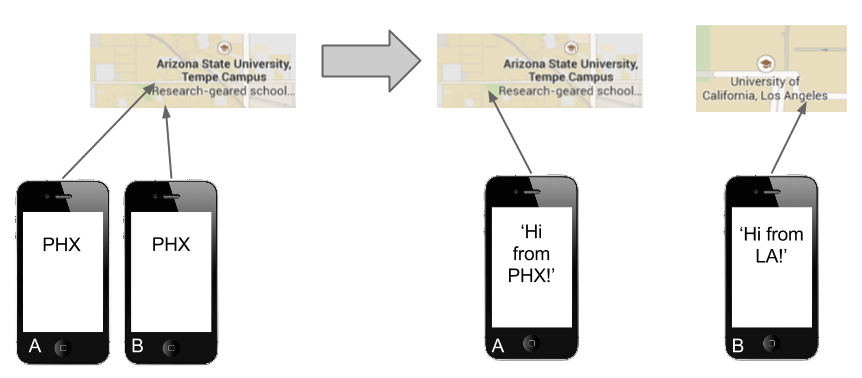
\includegraphics[width=.48\textwidth]{figs/zones}}
\caption{Chat example with zones.  When users are chatting in zones mode they will be able to chat in a zone even if they are not currently located in that zone. So for example if 2 users were present at ASU and afterwards one user went to UCLA  (or anywhere) they would still be able to communicate for a few days, because of their previous association with ASU.  }
\label{zones}
\end{figure}

\subsection{Server Side(Cloud Code \& Firebase)}
% Christophe, can you add more to what I have and maybe change so it doesn't sounds like we just copied and paste?
% URL for reference if needed, http://jormungand.net/projects/misc/em/
Most heavy lifting occurs on the server side where we have less limitations on resources.  In particular Parse allows processing in 15-second chunks on their high-performance distributed computing system, running a form of Javascript.  This means that if tasks can be parallelized easily they can run free, and also very very quickly.  As a result we discovered a Javascript implementation of the Expectation Maximization(EM) algorithm and modified it to work within the confines of Parse Cloud Code.  To handle the data flow we first pull all the user data down from Firebase, the users are returned as JSON objects. The user information is then stripped down to a time-series of locations, which are then separated and treated as a single time point. The location data is then passed into the EM algorithm to calculate clusters and user-cluster relationship.  Once the clusters are calculated the Google Places API is invoked to name the zones.  In practice We had significant difficulties getting intelligible results from Google Places API, ``ASU" became ``ASU Undergraduate Admissions" or ``ASU Museum", so zone names were manually curated.   It looks like the Google Places API would be appropriate to use when dealing with small zones, like a museum or stadium for a football game.  Or perhaps for very large zones such as "Tempe", but it seems to have significant difficulties when naming mid-sized zones.  After the zones are created they are pushed back into Firebase so that they can be accessed by users.  One implementation limitation is the transition of messages between zones.  When the zones are recreated it is probable that most zones will be fairly static (e.g. a generic ASU zone should be maintained),  so we should be able to create a measure of difference between gaussians (mean and covariance matrixes) to automatically reassign messages from relocated zones.  Similarly we don't currently allow for changes in the number of zones, which means that for a new zone to appear it needs to not only be strong enough to form, but it must also be a tighter zone than another currently existing zone.  This limitation could be overcome fairly easily by measuring a gradient-descent of the error as we add more zones to the clustering as described in~\cite{ray1999determination}.







 

\section{Results}
Currently, the user is able post and read messages and will display the correct zone according to the user's location. As you can see in the video, currently, in the system there are actually three zones, however, since we are currently in Tempe and we pretended that we had been to New York, therefore, you can only see zone0 (New York) an zone1 (Tempe). Also, messages within each zones are not visible in other zones and messages are uploaded instantly then pull down to and from our Firebase server, if other user are currently viewing the zone, he/she will see the update instantly. As for our server, we have successfully communicated between a cloud computing server, Cloud Code, and a cloud storage, Firebase. We were also able to implement the Expectation Maximization algorithm in JavaScript on Cloud Code and able to correctly cluster and name zones dynamically as the users move or get online. Even though they are two different systems, the lag time is barely noticeable. 


\section{Conclusion}
In this work we presented GeoChat, a novel chat application for the iPhone Operating System (iOS) allowing for geolocalized chat.  We discussed some of the challenges in implementation; including the transfer of data from high-response servers to compute and processing servers, limitations on accuracy of external API's, and difficulties intrinsic in the problem of grouping people only based on location.  We also demonstrate that complex behaviors in terms of locating zones and limiting chat between users can be achieved with a relatively simple database schema.

\subsection{Future Work}
This work presents a number of problems related to clustering users based only on location information, but there are many other problems that could be solved.  One such problems is how to deal with temporal artifacts such as whether a user has data for all points in a considered timeline.  Another possible opportunity for improvement is the slicing of the timeline to create higher-resolution zones.  For example when examining location-data across all time points we find a lower density of points than if we consider these zones only at the times when they are active.  For example the ASU campus has a higher density of people (users) during the day than are present at night, ignoring the effects of time introduces significant noise into the zone determination.  Finally, we don't have a way for users to maintain their zone membership.  If a user is actively communicating in a zone that they haven't been located in recently and a new zone calculation happens the user will be dropped from the zone, despite their participation in it.


\end{document}
	